\documentclass[11pt,reqno]{amsart}

% ---------------------------------------------------------------------------
%  The flagship integrative preprint.
%  A whole-repo, proof-status-honest exposition. Every result carries a
%  \status{} badge; the one GATED headline (SL(4) L=-M^4 / the A_n family) is
%  flagged in the abstract and in section 5; the physics arc is a FORCED
%  symmetry bridge plus a CONFIRMED dimensional wall, never a crossing to scale.
% ---------------------------------------------------------------------------

\usepackage{amsmath,amssymb,amsthm,mathtools}
\usepackage[T1]{fontenc}
\usepackage{lmodern}
\usepackage{microtype}
\usepackage{graphicx}
\usepackage[dvipsnames,table]{xcolor}
\usepackage{booktabs}
\usepackage{enumitem}
\usepackage[margin=1.05in]{geometry}
\usepackage[colorlinks=true,linkcolor=BlueViolet!70!black,citecolor=ForestGreen!60!black,urlcolor=NavyBlue]{hyperref}

\graphicspath{{figures/out/}}

% --- proof-status badges (mirror figures/style.mplstyle) -------------------
\definecolor{stProved}{HTML}{2E7D54}
\definecolor{stNum}{HTML}{1B3A5B}
\definecolor{stStruct}{HTML}{7A4F9E}
\definecolor{stKnown}{HTML}{8C8C8C}
\definecolor{stGated}{HTML}{B6411A}
\definecolor{stPost}{HTML}{C79A1E}

\newcommand{\badge}[2]{{\setlength{\fboxsep}{2pt}%
  \colorbox{#1}{\textcolor{white}{\sffamily\bfseries\scriptsize #2}}}}
\newcommand{\sProved}{\badge{stProved}{PROVED}}
\newcommand{\sExact}{\badge{stProved}{SYMBOLIC-EXACT}}
\newcommand{\sNum}{\badge{stNum}{NUMERICAL}}
\newcommand{\sStruct}{\badge{stStruct}{STRUCTURAL}}
\newcommand{\sKnown}{\badge{stKnown}{KNOWN}}
\newcommand{\sGated}{\badge{stGated}{GATED}}
\newcommand{\sPost}{\badge{stPost}{POSTULATED}}
\newcommand{\sForced}{\badge{stStruct}{FORCED}}

% --- theorem environments --------------------------------------------------
\theoremstyle{plain}
\newtheorem{theorem}{Theorem}[section]
\newtheorem{proposition}[theorem]{Proposition}
\newtheorem{lemma}[theorem]{Lemma}
\newtheorem{corollary}[theorem]{Corollary}
\newtheorem{conjecture}[theorem]{Conjecture}
\theoremstyle{definition}
\newtheorem{definition}[theorem]{Definition}
\newtheorem{observation}[theorem]{Observation}
\theoremstyle{remark}
\newtheorem{remark}[theorem]{Remark}

% --- macros ----------------------------------------------------------------
\newcommand{\SL}{\mathrm{SL}}
\newcommand{\GL}{\mathrm{GL}}
\newcommand{\PGL}{\mathrm{PGL}}
\newcommand{\tr}{\operatorname{tr}}
\newcommand{\Vol}{\operatorname{Vol}}
\newcommand{\CS}{\mathrm{CS}}
\newcommand{\C}{\mathbb{C}}
\newcommand{\R}{\mathbb{R}}
\newcommand{\Z}{\mathbb{Z}}
\newcommand{\Q}{\mathbb{Q}}
\newcommand{\Fp}{\mathbb{F}_p}
\newcommand{\kk}{\kappa}
\newcommand{\fig}[1]{Figure~\ref{#1}}
\DeclareMathOperator{\Sym}{Sym}

\begin{document}

\title[A self-generating object: tower, knot, and the boundary of scale]{A self-generating object:\\
the metallic once-punctured-torus family,\\ its trace-map tower, and the boundary between structure and scale}

\author{Dritëro M.}
\address{Independent researcher, Prishtina.}

\date{\today}

\begin{abstract}
We study a single object --- the metallic once-punctured-torus bundles, whose
monodromies are the words $R^mL^m$ in the two Dehn twists --- and follow it across
four mathematical registers: the dynamics of its trace map, the representation
theory of an associated tower, the geometry of the figure-eight knot's character
variety, and a duality of a four-dimensional gauge theory. The boundary invariant
$\kk=\tr[A,B]$ is exactly the Fricke--Vogt invariant of the Fibonacci trace map,
and the metallic monodromies realise the $\SL(2,\Z)$ mapping-class action on the
Fricke cubic. The adjoint-type tower factors over a Dickson catalogue
$\chi(\pm M^k)$, proved from first principles through $\SL(4)$. On the principal
Dehn-filling component the longitude and meridian eigenvalues satisfy
$L=(-1)^{n-1}M^n$; this reproduces Cooper--Long at $\SL(2)$ and Falbel at $\SL(3)$,
and gives $L=-M^4$ at $\SL(4)$, which we establish symbolic-exact and complete on
the irreducible locus. \textbf{The $\SL(4)$ result and the family it suggests are
flagged \sGated: after an adversarial literature read they appear novel but require
a specialist's confirmation, and the family is established only at $n=3,4$.}
Finally we make precise where the object reaches physics and where it stops: its
$\SL(2,\Z)$ symmetry \emph{is} the $S$-duality / mapping-class action of the
$\mathcal{N}=2^\ast$ class-$S$ theory (a forced identification, literature-confirmed),
yet no $\kk$-type or volume-type invariant carries a physical \emph{scale} across
that bridge. The pairing --- a real bridge, a confirmed wall --- is the honest
limit of how far a single self-generating object reaches. Every statement is tagged
by its proof status; nothing here is asserted beyond what a reader can check.
\end{abstract}

\maketitle

\section{Introduction: one object, four registers}
\label{sec:intro}

This paper is the report of a single sustained experiment. We fix one mathematical
object --- a family of hyperbolic three-manifolds so small and so forced that it is
hard to call it a choice --- and we follow it wherever its own structure leads. It
leads, as it turns out, into four different parts of mathematics: the dynamics of a
trace map, the representation theory of a tower of Lie groups, the geometry of the
figure-eight knot's character variety, and the duality group of a four-dimensional
supersymmetric gauge theory. The thesis of the paper is not any one of the results
along the way. It is that these four faces are faces of \emph{the same object}, and
that following the object honestly --- recording at every step exactly what is proved,
what is computed, what is borrowed, and what is merely suggested --- maps out precisely
how far such an object reaches, and where it stops.

\subsection*{A note on proof status} Because the object touches so many registers, the
single greatest risk is a quiet drift in what is being claimed. We therefore attach to
every substantive statement a colour-coded badge:
\begin{center}\small
\sProved\ exact and machine-checkable\quad
\sExact\ symbolic over a ring\quad
\sNum\ high-precision numerics\\[2pt]
\sStruct\ structurally forced, not fully symbolic\quad
\sKnown\ established in the literature\\[2pt]
\sGated\ appears new but awaits a specialist\quad
\sPost\ proposed, not put through the verification gate
\end{center}
The badges are not decoration. The one genuinely new headline of the paper --- the
$\SL(4)$ figure-eight $A$-polynomial $L=-M^4$ and the family it suggests
(Section~\ref{sec:knot}) --- carries the badge \sGated\ throughout: an adversarial
literature read found no prior art, but an AI-assisted read \emph{de-risks} a novelty
question without \emph{closing} it, and the family is established only at two values of
the rank. We state this in the abstract, we state it again here, and we state it at the
result. Everything else in the paper is \sProved, \sExact, \sNum, or \sKnown, and is
labelled accordingly.

\subsection{The motivating question, and the firewall that contains it}

The object was not chosen for its knot theory. It was chosen as the smallest answer to
a deliberately na\"ive question: \emph{what is the least structure that is not nothing?}
One can refuse the metaphysics of ``why is there something'' and ask instead, as a
mathematical question, what the minimal non-degenerate self-referential object looks
like --- and discover that the minimal answers do not form a unique point but a
\emph{self-generating family}. That reframing is the project's philosophical spine, and
we will let it motivate the exposition. But motivation is all it is. We adopt one
absolute rule, which we will call the \emph{firewall}:

\begin{quote}\itshape
Philosophy and physical interpretation may cite mathematics; mathematics may never cite
philosophy. If a motivating sentence is ever needed to support a theorem, the boundary
has been crossed, and the sentence is wrong where it stands.
\end{quote}

This is why the paper can be, at once, philosophically motivated and mathematically
sober. The reader who wants only the theorems may read Sections~\ref{sec:object}--\ref{sec:chirality}
and ignore every interpretive remark without losing a single implication. The reader
interested in the larger question will find it addressed exactly once, in
Section~\ref{sec:bridge}, and addressed by the same standard of proof as everything
else: with a forced mathematical identification on one side and a confirmed obstruction
on the other.

\subsection{Architecture, not furniture}

A second principle organises what we do and do not claim. The object is a theory of
\emph{structure} --- of symmetry, of hierarchy, of which configurations are possible ---
and not a theory of \emph{values}: it does not select a coupling constant, a mass, or a
cosmological scale. Borrowing a phrase from the project's notes, it is architecture, not
furniture. This is not modesty for its own sake; it is a theorem-shaped fact, made
precise in Section~\ref{sec:bridge}, that the invariants the object naturally produces
are dimensionless and scale-free. Stating it at the outset pre-sorts the questions one
may ask: structural questions (what is the symmetry? what is the representation? what is
the $A$-polynomial?) have answers, and we give them; value questions (what number does
this predict?) meet a wall, and we exhibit the wall rather than climbing over it.

\subsection{What is in the paper}

Section~\ref{sec:object} introduces the metallic once-punctured-torus bundles and their
arithmetic. Section~\ref{sec:invariant} pins the boundary invariant $\kk=\tr[A,B]$ to
the Fricke--Vogt invariant of the Fibonacci trace map and identifies the metallic
monodromies with the $\SL(2,\Z)$ mapping-class action. Section~\ref{sec:tower} builds
the adjoint-type ``Dickson tower'' and proves its factorisation through $\SL(4)$, noting
the precise wall at $n\ge 5$. Section~\ref{sec:knot} is the geometric heart: the
trace-map fixed locus reproduces the figure-eight $A$-polynomial exactly at $\SL(2)$ and
$\SL(3)$, and yields the new, gated $\SL(4)$ relation $L=-M^4$, complete on the
irreducible locus. Section~\ref{sec:chirality} closes the chirality question with a
palindromic criterion for amphichirality. Section~\ref{sec:bridge} makes the bridge to
physics and confirms the wall. Sections~\ref{sec:discussion}--\ref{sec:open} discuss the
object's proper name as an aperiodic-order operator, the open problems, and the
reproducibility discipline; an appendix collects proof sketches.

\section{The object: metallic once-punctured-torus bundles}
\label{sec:object}

Let $T_\circ$ be the once-punctured torus and $\mathrm{MCG}(T_\circ)\cong\SL(2,\Z)$ its
mapping class group, generated by the two Dehn twists $R$ and $L$ along a dual pair of
simple closed curves. To a pseudo-Anosov word $\varphi$ in $R$ and $L$ one associates
the mapping torus $M_\varphi = T_\circ\times[0,1]/(x,1)\sim(\varphi x,0)$, a cusped
hyperbolic three-manifold fibring over the circle. Our object is the subfamily whose
monodromies are the \emph{metallic words}
\begin{equation}
  W_m \;=\; R^m L^m,\qquad m=1,2,3,\dots
\end{equation}
together with their cusp-glued composites $R^{m_1}L^{m_1}\cdots R^{m_k}L^{m_k}$, which we
return to in Section~\ref{sec:chirality}.

\subsection{Why ``metallic''}

In the standard representation $R\mapsto\left(\begin{smallmatrix}1&1\\0&1\end{smallmatrix}\right)$,
$L\mapsto\left(\begin{smallmatrix}1&0\\1&1\end{smallmatrix}\right)$ of
$\mathrm{MCG}(T_\circ)$, a single metallic block is conjugate to a power of the matrix
\begin{equation}
  M_m \;=\; \begin{pmatrix} m & 1 \\ 1 & 0 \end{pmatrix},
  \qquad \det M_m = -1,\qquad \tr M_m = m,
\end{equation}
whose larger eigenvalue is the \emph{metallic mean}
$\lambda_m=\tfrac12\!\left(m+\sqrt{m^2+4}\right)$, the positive solution of the
self-referential equation $x = m + 1/x$. For $m=1$ this is the golden mean
$\varphi=\tfrac12(1+\sqrt5)$; for $m=2$ the silver mean $1+\sqrt2$. The dilatation of the
pseudo-Anosov monodromy $W_m$ is $\lambda_m^2$; the larger $m$, the more strongly the
fibre is stretched (\fig{fig:metallic}).

\begin{figure}[t]
  \centering
  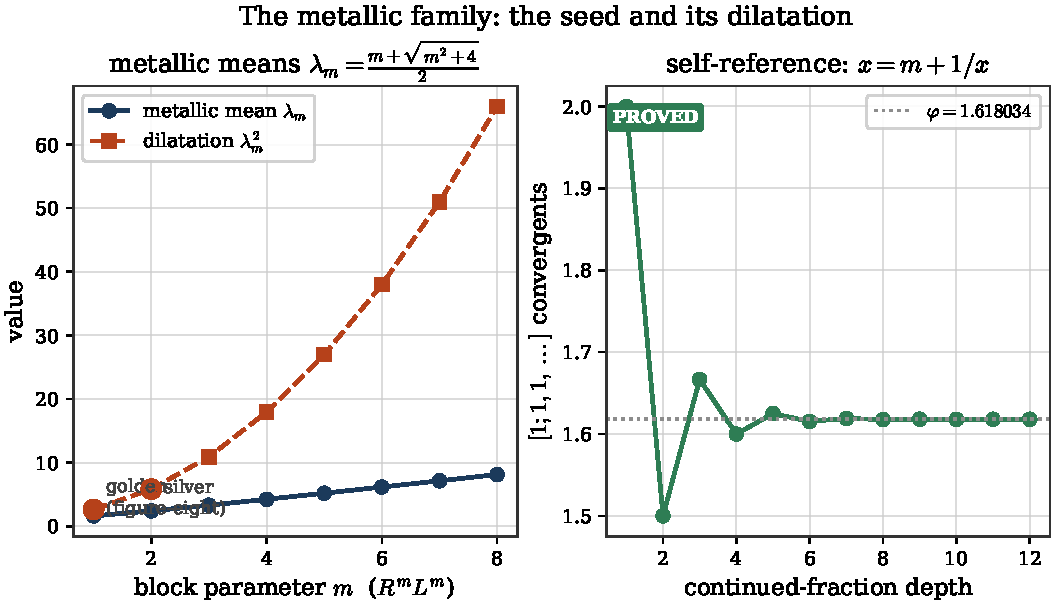
\includegraphics[width=\linewidth]{fig01_metallic_means}
  \caption{The metallic seeds. \emph{Left:} the metallic mean $\lambda_m$ and the
  monodromy dilatation $\lambda_m^2$ as functions of the block parameter $m$; the
  golden ($m=1$, figure-eight) and silver ($m=2$) cases are marked. \emph{Right:} the
  self-referential recursion $x=m+1/x$ converging to $\varphi$ --- the object literally
  generated by iterating a minimal self-reference. \sProved}
  \label{fig:metallic}
\end{figure}

The determinant $\det M_m=-1$ is not incidental; it is the source of the
orientation-reversing structure that will govern chirality in Section~\ref{sec:chirality}
and the alternating sign $(-1)^{n-1}$ in the $A$-polynomial family of
Section~\ref{sec:knot}. We record it as the object's first structural fact.

\begin{observation}[\sProved]
The eigenvalues of $M_m^{-1}$ coincide with those of $-M_m$. Indeed if $\lambda,\mu$ are
the eigenvalues of $M_m$ then $\lambda\mu=\det M_m=-1$, so $\lambda^{-1}=-\mu$ and
$\mu^{-1}=-\lambda$; hence $\chi(M_m^{-1})=\chi(-M_m)$ as characteristic polynomials.
This identity is why the ``inverse'' and ``sign'' directions of the tower
(Section~\ref{sec:tower}) coincide.
\end{observation}

\subsection{The figure-eight as the golden case}

The case $m=1$ is the figure-eight knot complement $4_1$. Its monodromy is
$\varphi=R L$, conjugate to $M_1^2=\left(\begin{smallmatrix}2&1\\1&1\end{smallmatrix}\right)$,
and it is the unique arithmetic once-punctured-torus bundle of smallest volume,
$\Vol(4_1)=2.029883\ldots=2V_{\mathrm{tet}}$, with invariant trace field $\Q(\sqrt{-3})$.
It is amphichiral (it admits an orientation-reversing self-homeomorphism), and its
Chern--Simons invariant vanishes. These two facts --- minimality and amphichirality ---
make the figure-eight the natural \emph{base} of the family, and, as we will see in
Section~\ref{sec:bridge}, the object \emph{least} able to carry a physical scale. The
silver case $m=2$ is the bundle with monodromy $R^2L^2$, trace field $\Q(i)$, the second
and last arithmetic member of the canonical metallic series.

\subsection{Trace fields and the arithmetic backbone}

The monodromy matrix $M_m$ has real eigenvalues lying in the quadratic field
$\Q(\sqrt{m^2+4})$. This is the field of the \emph{dynamics} --- the dilatation field ---
and is distinct from the invariant trace field of the hyperbolic structure on $M_{W_m}$,
which is in general a complex field (e.g.\ $\Q(\sqrt{-3})$ for the figure-eight). Keeping
these two fields apart is a recurring discipline of the subject; we use the dilatation
field $\Q(\sqrt{m^2+4})$ whenever we speak of the trace-map dynamics, and name the
invariant trace field explicitly when we mean the hyperbolic geometry. The arithmetic
backbone of the canonical family is summarised in Table~\ref{tab:fields}.

\begin{table}[h]
\centering\small
\begin{tabular}{cllll}
\toprule
$m$ & word & metallic mean & dilatation field & note \\
\midrule
$1$ & $RL$ & golden $\varphi$ & $\Q(\sqrt5)$ & figure-eight $4_1$; trace field $\Q(\sqrt{-3})$ \\
$2$ & $R^2L^2$ & silver $1+\sqrt2$ & $\Q(\sqrt8)$ & ``silver'' bundle; trace field $\Q(i)$ \\
$m$ & $R^mL^m$ & $\tfrac12(m+\sqrt{m^2+4})$ & $\Q(\sqrt{m^2+4})$ & generic metallic bundle \\
\bottomrule
\end{tabular}
\caption{The arithmetic backbone of the canonical metallic family. \sProved}
\label{tab:fields}
\end{table}

\section{The invariant: $\kk=\tr[A,B]$ and the Fricke cubic}
\label{sec:invariant}

A representation $\rho\colon\pi_1(T_\circ)=\langle A,B\rangle\to\SL(2,\C)$ of the free
group on two generators is determined up to conjugacy by the three trace coordinates
\begin{equation}
  x=\tr\rho(A),\qquad y=\tr\rho(B),\qquad z=\tr\rho(AB),
\end{equation}
a classical theorem of Fricke and Vogt. In these coordinates the trace of the boundary
commutator is the \emph{Fricke cubic}
\begin{equation}\label{eq:fricke}
  \kk \;=\; \tr\rho[A,B] \;=\; x^2+y^2+z^2-xyz-2,
\end{equation}
and the relative character variety of $T_\circ$ with fixed boundary holonomy is the level
surface $\{\kk=\text{const}\}$, an affine cubic surface (\fig{fig:fricke}). The mapping
class group acts on the trace coordinates by polynomial automorphisms preserving
\eqref{eq:fricke} leaf by leaf; this is the \emph{trace map}.

\begin{figure}[t]
  \centering
  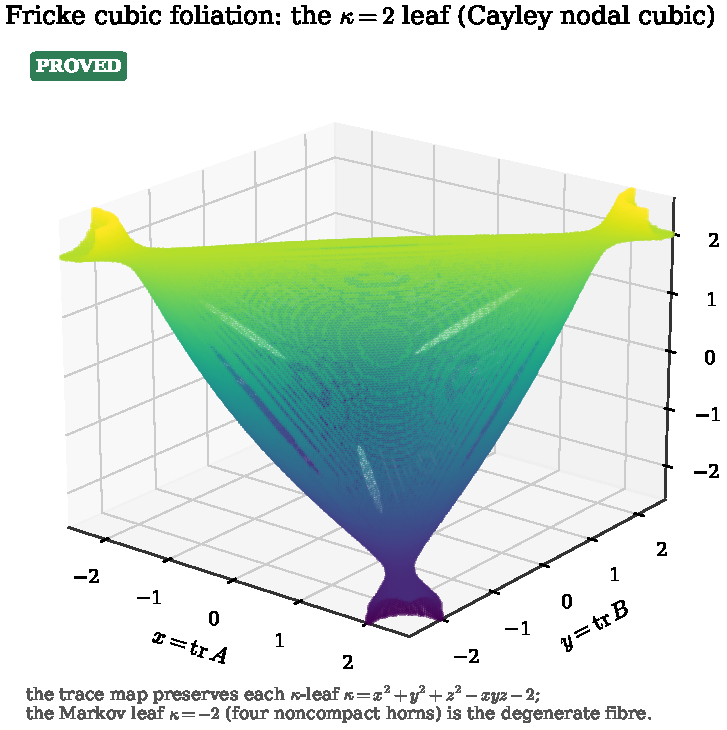
\includegraphics[width=0.82\linewidth]{fig02_fricke_cubic}
  \caption{A leaf of the Fricke cubic foliation $\kk=x^2+y^2+z^2-xyz-2$: the
  $\kk=2$ leaf is the classical Cayley nodal cubic, with four conical nodes (marked).
  The trace map preserves each $\kk$-leaf; the Markov leaf $\kk=-2$ (four noncompact
  horns) is the degenerate fibre on which the dynamics is most rigid. \sProved}
  \label{fig:fricke}
\end{figure}

\subsection{$\kk$ is the Fricke--Vogt invariant of the Fibonacci trace map}

The cubic \eqref{eq:fricke} is exactly the conserved quantity of the Fibonacci trace map
of Kohmoto--Kadanoff--Tang and S\"ut\H{o} \cite{kkt1983,suto1987}. In the half-trace
normalisation $x=2X$ etc., one has the identity
\begin{equation}\label{eq:kfv}
  \kk \;=\; 4\,I_{\mathrm{FV}} + 2,
  \qquad I_{\mathrm{FV}} = X^2+Y^2+Z^2-2XYZ-1,
\end{equation}
where $I_{\mathrm{FV}}$ is the Fricke--Vogt invariant familiar from the spectral theory
of the Fibonacci Hamiltonian. We verified \eqref{eq:fricke}--\eqref{eq:kfv} and the
following statements symbolically.

\begin{proposition}[\sProved]\label{prop:invariant}
Let $\tau_a,\tau_b$ be the trace-map automorphisms induced by the two Dehn twists. Then:
\begin{enumerate}[leftmargin=2em]
\item $\tau_a$ and $\tau_b$ preserve $\kk$ identically, so the metallic monodromies
  $W_m=R^mL^m$ act on each Fricke leaf; the action on trace coordinates \emph{is} the
  $\SL(2,\Z)$ mapping-class action on the character variety.
\item The leaf $\kk=-2$ is the \emph{Markov surface} $x^2+y^2+z^2=xyz$, on which the
  metallic dynamics restricts to the classical Markov triple recursion.
\item On the leaf carrying the metallic monodromy the eigenvalue of the linearised action
  is $\lambda_m^2$, the dilatation; the fixed slopes are the roots of $t^2+mt-1=0$, and
  the dynamical degree (in the sense of Cantat--Loray \cite{cantatloray2009}) equals
  $\lambda_m^2$.
\end{enumerate}
\end{proposition}

The content of Proposition~\ref{prop:invariant} is that three a priori different objects
--- the boundary trace of a surface-group representation, the conserved invariant of a
one-dimensional aperiodic Schr\"odinger operator, and the Markov cubic of number theory
--- are literally the same polynomial, and that the metallic monodromies are the
mapping-class symmetry of all three at once. None of these identifications is new
individually (they go back to Fricke, to KKT/S\"ut\H{o}, and to Markov; see
\cite{goldman2009,baakegrimm2013,aigner2013}); the point is that they are properties of
\emph{this} object, holding simultaneously, and we make them the anchor for everything
downstream.

\subsection{The trace map as a dynamical system}

Iterating the trace map on a Fricke leaf gives a polynomial dynamical system whose
fixed point structure encodes the object's rigidity. At the distinguished fixed point ---
the ``void'' from which the family is generated --- the linearisation is a hyperbolic
saddle with one marginal direction: the Lyapunov spectrum is
$\{0,\,\pm 4\log\varphi\}$ for the golden case (\fig{fig:dynamics}). The single zero
exponent is the direction along the Fricke leaf; the two nonzero exponents are the
expanding/contracting directions of the metallic stretch. This is the dynamical face of
the object; its representation-theoretic face is the subject of the next section.

\begin{figure}[t]
  \centering
  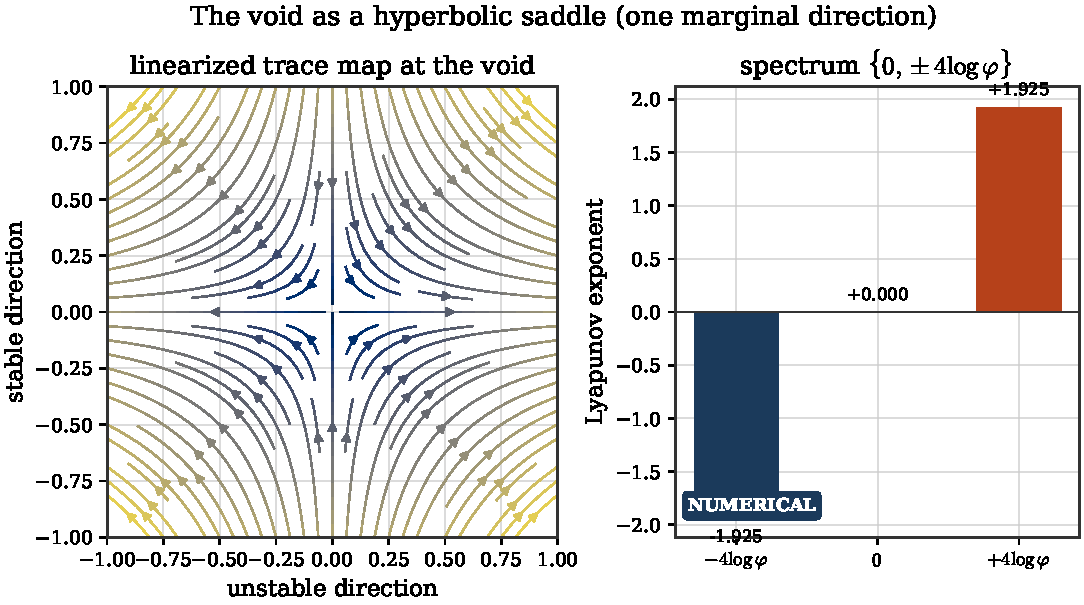
\includegraphics[width=\linewidth]{fig03_trace_map_dynamics}
  \caption{The void fixed point of the metallic trace map. \emph{Left:} the linearised
  flow, a hyperbolic saddle with one marginal (leaf) direction. \emph{Right:} the
  Lyapunov spectrum $\{0,\pm 4\log\varphi\}$ of the golden case. \sNum}
  \label{fig:dynamics}
\end{figure}

\section{The tower: a Dickson factorisation, proved through $\SL(4)$}
\label{sec:tower}

The trace map of Section~\ref{sec:invariant} lives on $\SL(2,\C)$ characters. Replacing
$\SL(2,\C)$ by $\SL(n,\C)$ produces, for each $n$, an $(n^2-1)$-dimensional linear map
$J(m)$ --- the linearisation of the $\SL(n)$ metallic trace map at the trivial
representation, an adjoint-type representation of the external monodromy. The
\emph{tower} is the sequence $(J(m))_{n\ge2}$, and its arithmetic is governed by a single
catalogue.

\subsection{The Dickson catalogue}

For the metallic matrix $M=M_m$ write $L_k=\tr(M^k)$, the Lucas-type sequence with
$L_k=mL_{k-1}+L_{k-2}$ (recall $\det M=-1$). The characteristic polynomial of $\pm M^k$
is
\begin{equation}
  \chi(\pm M^k) \;=\; t^2 \mp L_k\,t + (-1)^k,
\end{equation}
a \emph{Dickson polynomial} in the variable $m$. The central structural fact is that the
$(n^2-1)$-dimensional charpoly $\det(tI-J(m))$ factors entirely over this catalogue.

\begin{theorem}[\sExact, \sProved]\label{thm:tower}
Over $\Z[m]$ one has the factorisations
\begin{align}
  n=3:\quad \det(tI-J) &= \chi(M^{-1})\,\chi(M^2)\,\chi(M^3)\,(t-1)(t+1),\\
  n=4:\quad \det(tI-J) &= \chi(M)\,\chi(-M)\,\chi(M^2)\,\chi(-M^2)\,\chi(M^3)\,\chi(M^4)\,(t-1)^2(t+1).
\end{align}
The $n=3$ identity is symbolic over all $m$; the $n=4$ identity is established
\emph{from first principles} by a Chinese-remainder/$\Fp$ interpolation of the symbolic
Jacobian over $\Z[m]$, with the factored characteristic polynomial reconstructed exactly
and verified to match the catalogue.
\end{theorem}

Figure~\ref{fig:tower} displays the catalogue: each factor $\chi(\pm M^k)$ is a node at
signed power $k$, coloured by the parity of $|k|$. (By the Observation of
Section~\ref{sec:object}, $\chi(M^{-1})=\chi(-M)$, so the $n=3$ ``inverse'' node and a
sign node coincide.) The parity colouring is itself a theorem.

\begin{figure}[t]
  \centering
  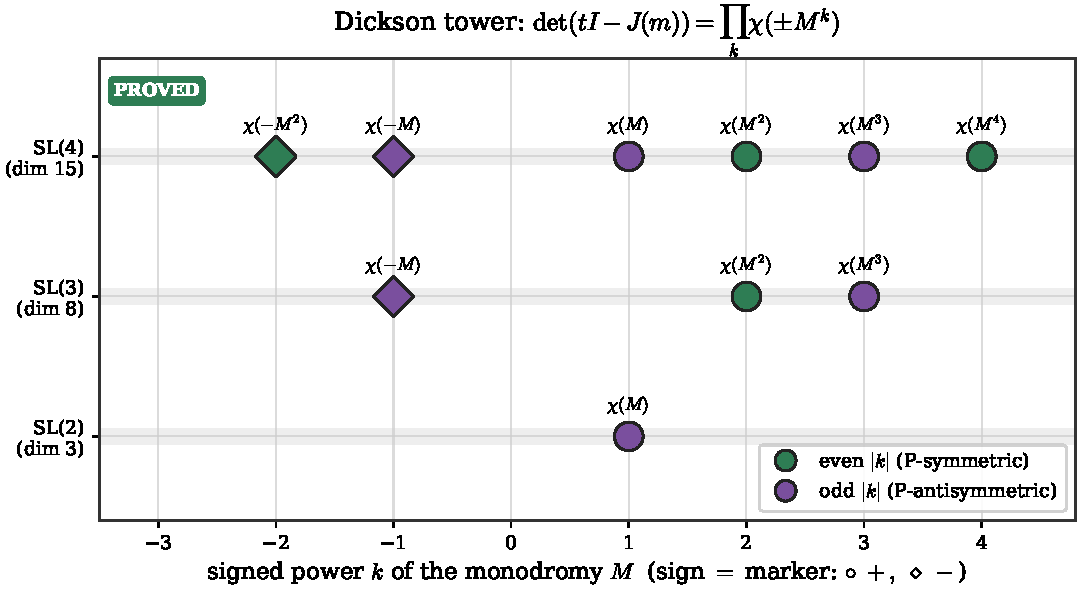
\includegraphics[width=\linewidth]{fig04_dickson_tower}
  \caption{The Dickson tower. The $(n^2-1)$-dimensional charpoly $\det(tI-J(m))$ factors
  into Dickson pieces $\chi(\pm M^k)=t^2\mp L_k t+(-1)^k$; nodes are placed at the signed
  power $k$ and coloured by parity ($\circ$ sign $+$, $\diamond$ sign $-$). Even-$|k|$
  factors are $P$-symmetric, odd-$|k|$ factors $P$-antisymmetric --- the same
  $\theta=-w_0$ that grades $A_{n-1}$. Data and factorisation from the symbolic
  $\SL(4)$ Jacobian. \sProved}
  \label{fig:tower}
\end{figure}

\begin{proposition}[\sProved]\label{prop:parity}
The factor $\chi(M^k)$ sits in the $P$-symmetric part of the adjoint module when $|k|$ is
even and in the $P$-antisymmetric part when $|k|$ is odd, where $P$ is the
contragredient ($m\mapsto -m$) symmetry. This grading is exactly the action of the
opposition involution $\theta=-w_0$ of the root system $A_{n-1}$ (\fig{fig:opp}); it
holds for all $n$ by a Dickson-parity argument and requires no numerics.
\end{proposition}

\begin{figure}[t]
  \centering
  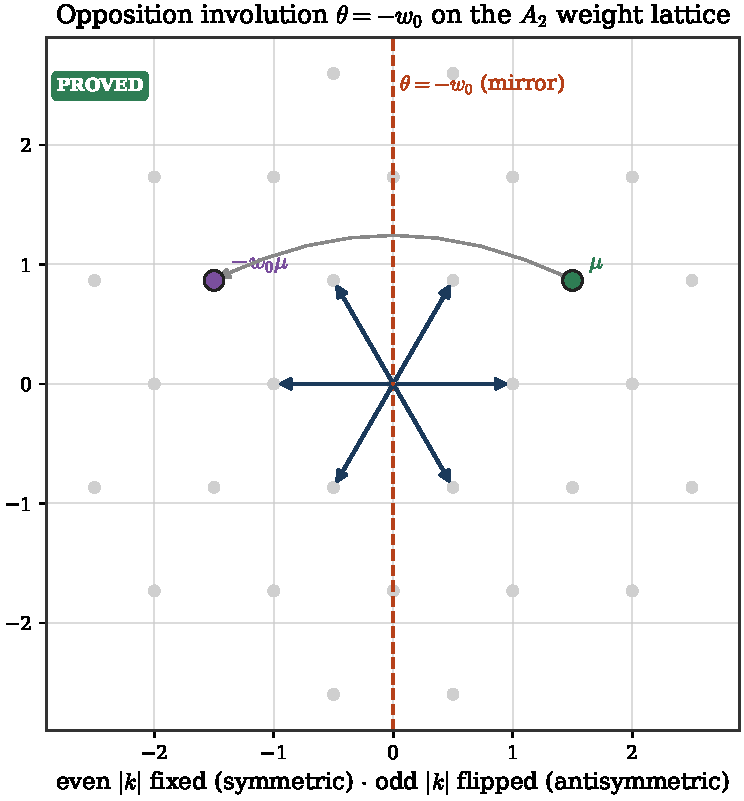
\includegraphics[width=0.62\linewidth]{fig05_opposition_involution}
  \caption{The opposition involution $\theta=-w_0$ on the $A_2$ (i.e.\ $\SL(3)$) weight
  lattice: a weight $\mu$ and its image $-w_0\mu$ are exchanged by the mirror. Even-$|k|$
  Dickson factors are fixed (symmetric), odd-$|k|$ flipped (antisymmetric). The same
  involution governs charge conjugation of the $W_N$ algebras. \sProved}
  \label{fig:opp}
\end{figure}

\subsection{The wall at $n\ge5$}

The factorisation is proved for $n\le4$ and is \emph{structurally} understood, but not
symbolically proved, for $n\ge5$. The obstruction is sharp and worth stating precisely,
because it is the paper's principal open problem (Section~\ref{sec:open}). One can write
the tower abstractly as a symmetric-power decomposition
\begin{equation}\label{eq:symw}
  \rho_n \;\cong\; \Sym^n(W)\;\oplus\;\bigl(\Sym^{\,n-3}(W)\ominus W\bigr),
  \qquad W = V\oplus\mathbf{1},\ \det W=-1,
\end{equation}
with $W$ the external-monodromy fundamental; this is proved as an isomorphism of modules
at $n=3,4$ and conjectured in general. The remaining step --- assembling the bounded
rank-one $e_2/\Lambda^2$ closure into the exact trace map as a \emph{functorial}
construction --- is genuinely open. We emphasise that three plausible shortcuts are
\emph{dead}: a perturbative numerical route does not converge at the doubly-degenerate
$\chi(M^2)^2$ sector that first appears at $n=5$; the $\Lambda^2$ functoriality, while
real, does not break that degeneracy; and a cohomological route returns the trivial-rep
fixed line rather than the tower. The principal-spectrum analysis explains why $n=5$ is a
threshold rather than a mere computational limit: the Dehn-filling boundary condition
forces the principal spectrum to degenerate there (Section~\ref{sec:knot}), so
``exponent $=$ rank'' is an $n\in\{3,4\}$ phenomenon, not a failure of effort.

\section{The knot: the figure-eight $A$-polynomial family}
\label{sec:knot}

We now turn to the geometric face of the object: the figure-eight knot complement and its
$A$-polynomial. The $A$-polynomial records the relation between the meridian eigenvalue
$M$ and the longitude eigenvalue $L$ as the cusp holonomy varies along the character
variety. The central observation is that the trace-map fixed locus of the previous
sections \emph{reproduces} the published $A$-polynomial data exactly at $\SL(2)$ and
$\SL(3)$, and \emph{extends} it to $\SL(4)$.

\subsection{The known base cases}

\begin{theorem}[\sKnown, reproduced exactly]\label{thm:cl}
At $\SL(2)$ the fixed locus $\mathrm{Fix}(T_1^2)$ of the squared metallic trace map
yields the Cooper--Long figure-eight $A$-polynomial \cite{ccgls1994}
\begin{equation}\label{eq:CL}
  A(M,L) = M^4L^2 + (-M^8+M^6+2M^4+M^2-1)\,L + M^4,
\end{equation}
to machine precision. At $\SL(3)$ the same construction reproduces the boundary
$A$-variety of Heusener--Mu\~noz--Porti and Falbel et al.\
\cite{hmp2016,fgkrt2014}: the two Dehn-filling components
$W_1:\ M^3=L$ and $W_2:\ M^3L=1$, together with a geometric component $V_0$ (the
$\Sym^2$ shadow of the $\SL(2)$ component) which has no tidy closed form.
\end{theorem}

Figures~\ref{fig:apoly} and \ref{fig:sl3} show the $\SL(2)$ curve and the $\SL(3)$
component structure. We claim no novelty for Theorem~\ref{thm:cl}: it is a verification
that our trace-map machinery agrees with the literature, and it is the control that
licenses the extension to $\SL(4)$.

\begin{figure}[t]
  \centering
  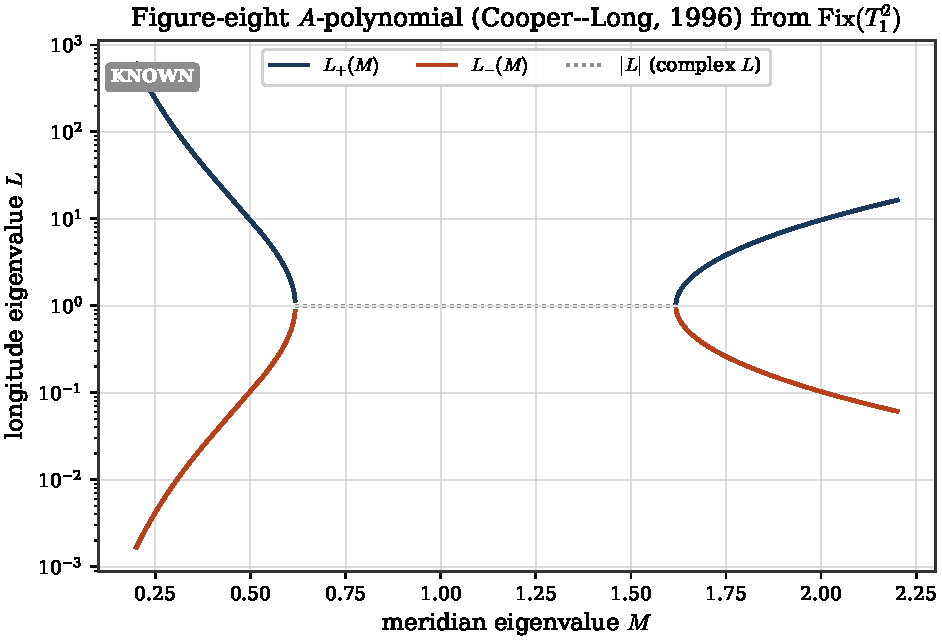
\includegraphics[width=0.78\linewidth]{fig06_apolynomial_sl2}
  \caption{The figure-eight $A$-polynomial \eqref{eq:CL} (Cooper--Long) recovered from
  the trace-map fixed locus: the two real branches $L_\pm(M)$ and, in the complex-$L$
  region, $|L|=1$. \sKnown}
  \label{fig:apoly}
\end{figure}

\begin{figure}[t]
  \centering
  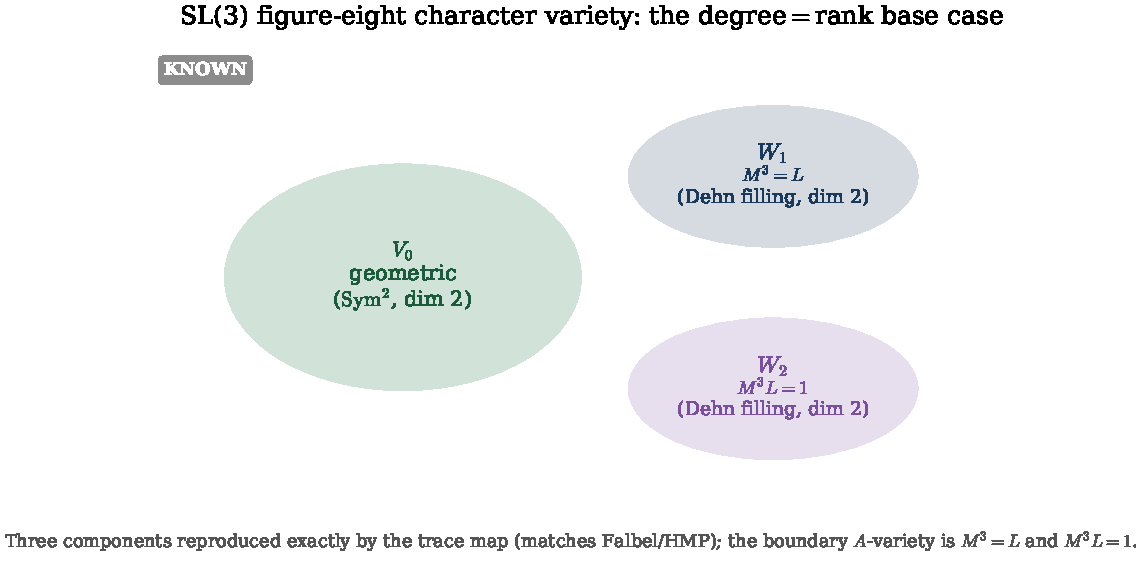
\includegraphics[width=0.82\linewidth]{fig07_sl3_character_variety}
  \caption{The $\SL(3)$ figure-eight character variety reproduced by the trace map: the
  geometric component $V_0$ ($\Sym^2$, dimension $2$) and the two Dehn-filling components
  $W_1:M^3=L$, $W_2:M^3L=1$, matching Falbel et al.\ and Heusener--Mu\~noz--Porti. This
  is the $n=3$ base case of the degree$=$rank family. \sKnown}
  \label{fig:sl3}
\end{figure}

\subsection{The $\SL(4)$ relation, and the family it suggests}

On the principal Dehn-filling component --- the component on which $\tr A=\tr A^{-1}=1$,
which carries the geometric representation --- the boundary eigenvalues satisfy a single
clean relation, the meridian raised to the rank:
\begin{equation}\label{eq:family}
  L \;=\; (-1)^{\,n-1} M^{\,n}.
\end{equation}
At $n=2$ this is the effective slope of \eqref{eq:CL}; at $n=3$ it is Falbel's $L=+M^3$.
The new instance is $n=4$.

\begin{theorem}[\sExact \;/\; \sGated]\label{thm:m4l}
On the principal $\SL(4)$ Dehn-filling component the longitude and meridian eigenvalues
satisfy
\begin{equation}
  L = -M^4,
\end{equation}
established symbolic-exact over $\Q(\omega)$ ($\omega$ a primitive cube root of unity).
Concretely, eliminating the second generator collapses the bundle relations to an ideal
whose principal-spectrum stratum is a four-parameter family on which the identity
$[A,B]\cdot\det(t)^2 = -\det(t)\cdot\mu^4$ holds as a polynomial identity --- no division,
no numerics. Moreover this family is \emph{complete} on the irreducible locus
(Theorem~\ref{thm:complete}).
\end{theorem}

\paragraph{\textmd{\textbf{The gate, stated plainly.}}} Theorem~\ref{thm:m4l} is the one
result in this paper we cannot present as settled-novel, and we flag it \sGated\
deliberately and repeatedly. An adversarial literature read --- assuming the result was
already known and hunting for prior art in the Cooper--Long, Heusener--Mu\~noz--Porti,
Falbel, Tillmann and Bergeron--Falbel--Guilloux circle \cite{ccgls1994,hmp2016,fgkrt2014,tillmann2005,bfg2014}
--- found no statement of the $\SL(4)$ figure-eight $A$-polynomial $L=-M^4$, and the
literature describes $\SL(4)$ figure-eight geometry as open. But two cautions are
binding. \emph{First}, an AI-assisted literature read \emph{de-risks} a novelty question;
it does not \emph{close} it. The reader should treat ``appears novel'' as ``no prior art
was found by a non-specialist sweep,'' and the genuine verdict awaits a specialist in the
Falbel / Bergeron--Falbel--Guilloux subfield. \emph{Second}, the relation \eqref{eq:family}
is established only at $n=3$ (known) and $n=4$ (Theorem~\ref{thm:m4l}); the principal
$\SL(5)$ representation is not numerically locatable, so ``a family for all $n\ge3$'' is a
\emph{conjecture plus a prediction}, not an established family (\fig{fig:slope}). It may
also be implicit in the flag-variety frameworks of \cite{bfg2014,gtz2015}; that, too, is
for a specialist to decide.

\begin{figure}[t]
  \centering
  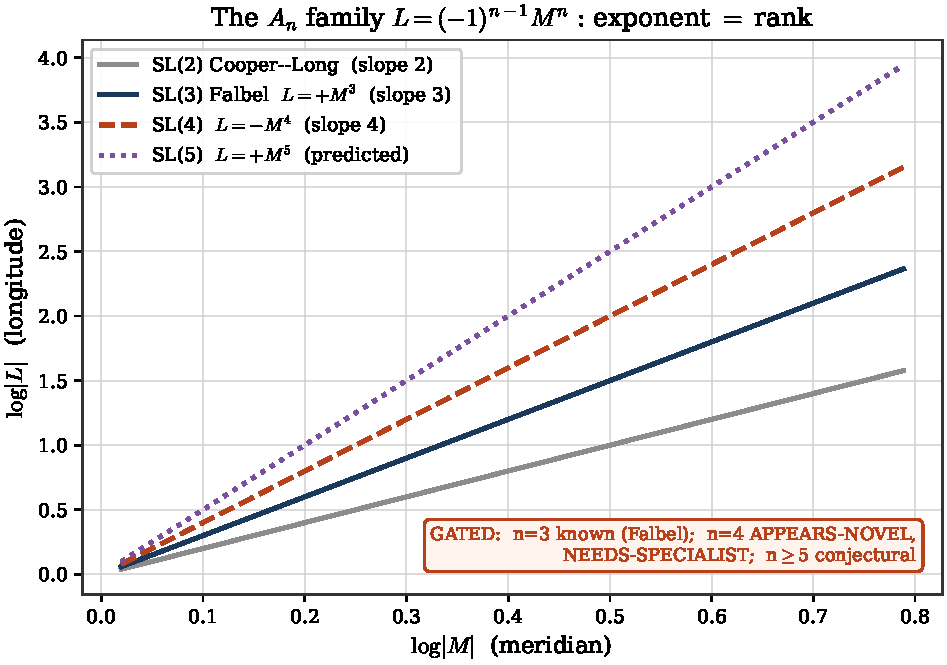
\includegraphics[width=0.78\linewidth]{fig08_an_family_slope_rank}
  \caption{The conjectural $A_n$ family $L=(-1)^{n-1}M^n$ in the $(\log|M|,\log|L|)$
  plane: the slope of each line equals the rank. $n=3$ is Falbel (known); $n=4$
  ($L=-M^4$) is Theorem~\ref{thm:m4l}, \sGated; $n\ge5$ is conjectural and not yet
  locatable. \sGated}
  \label{fig:slope}
\end{figure}

\subsection{Completeness on the irreducible locus}

The proof of $L=-M^4$ posits an explicit four-parameter family of $\SL(4)$ bundle
representations. A natural worry is that this family is only a checked corner of a larger
variety. It is not.

\begin{theorem}[\sProved]\label{thm:complete}
For the principal $A$-spectrum $\{1,1,\omega,\omega^2\}$, the defining ideal of the
$\SL(4)$ figure-eight bundle representations, stratified by the rank of the coupling
block (the only stratification compatible with the gauge action), has a single stratum
carrying absolutely irreducible representations: the four-parameter family of
Theorem~\ref{thm:m4l}. Every other stratum is reducible or vacuous ($\det t=0$).
Consequently $L=-M^4$ holds \emph{unconditionally on the irreducible locus}.
\end{theorem}

Figure~\ref{fig:strat} shows the stratification. The irreducibility classification was
performed exactly over a finite field using the \emph{Burnside} criterion (the generated
algebra is the full matrix algebra iff the representation is absolutely irreducible),
\emph{validated against} a stratum already proved reducible by hand. We stress this point
of method because the verdict flipped twice under scrutiny before settling: a tempting
alternative test, the Schur commutant, is \emph{invalid} for non-semisimple
representations and falsely flagged a provably-reducible stratum as irreducible. The
banked result rests on the validated test, not the convenient one.

\begin{figure}[t]
  \centering
  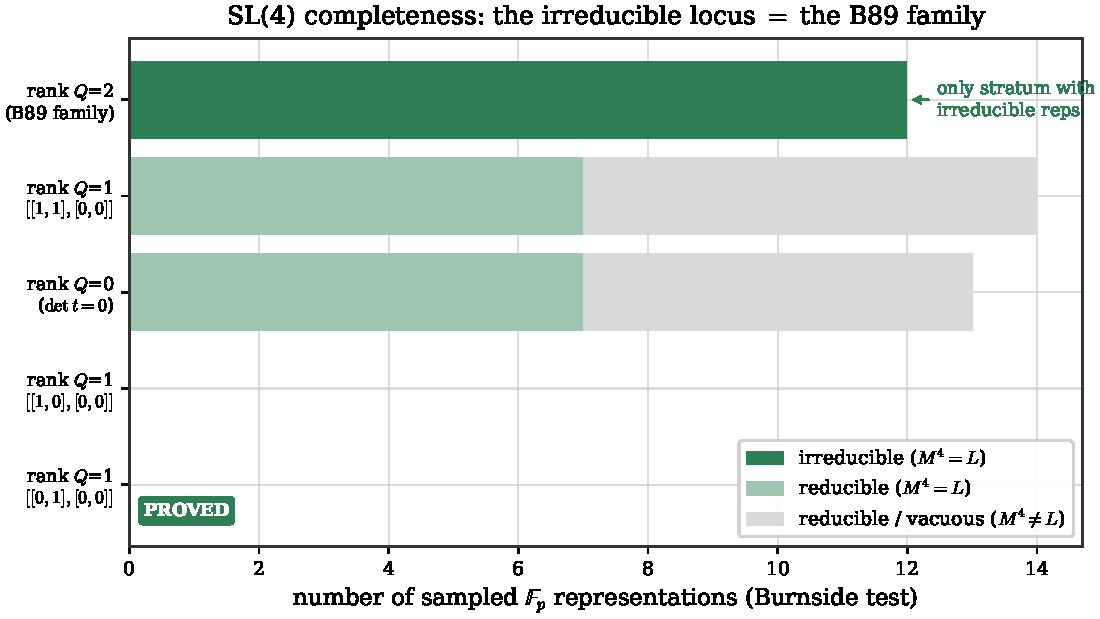
\includegraphics[width=\linewidth]{fig09_sl4_stratification}
  \caption{$\SL(4)$ completeness. Gauge-rank strata of the bundle ideal, classified by
  the Burnside test over $\Fp$: only the rank-$Q{=}2$ stratum (the family of
  Theorem~\ref{thm:m4l}) carries irreducible representations, and all of them satisfy
  $M^4=L$. The irreducible locus \emph{is} the family. \sProved}
  \label{fig:strat}
\end{figure}

\subsection{Why ``exponent $=$ rank'' stops}

The relation \eqref{eq:family} ties the $A$-polynomial exponent to the rank $n$, and the
sign $(-1)^{n-1}$ to $\det M=-1$. The mechanism is the principal Dehn-filling spectrum:
the boundary condition $\tr A=\tr A^{-1}=1$ \emph{forces} the spectrum to be
$\{1,i,-i\}$ at $n=3$, $\{1,1,\omega,\omega^2\}$ at $n=4$, and $\{1,1,1,-1,-1\}$ at
$n=5$; for $n\ge6$ it is impossible. At $n=5$ the forced spectrum makes $A^2=I$, hence
$\langle A,B\rangle$ dihedral, hence reducible --- there is no irreducible bundle
representation on the principal $\SL(5)$ component. So ``exponent $=$ rank'' is genuinely
an $n\in\{3,4\}$ phenomenon, read off the cusp's forced spectrum, and the apparent ceiling
is a fact about the boundary condition, not a limit of computation.

\section{Chirality: a palindromic criterion for amphichirality}
\label{sec:chirality}

The project's one \emph{proven} obstruction to Standard-Model-like structure is chirality:
parity violation requires a preferred handedness, and we can ask precisely whether the
metallic construction admits one. The answer, developed across a sub-arc of the work, is
a clean dichotomy.

\subsection{The block-length criterion}

Recall the composites $W=R^{m_1}L^{m_1}\cdots R^{m_k}L^{m_k}$. Each is a hyperbolic
once-punctured-torus bundle, and we ask when $M_W$ is amphichiral.

\begin{theorem}[\sProved \;(corollary of \cite{ghh2008})]\label{thm:palindrome}
The metallic composite with block-length sequence $(m_1,\dots,m_k)$ is amphichiral if and
only if the sequence is a \emph{cyclic palindrome}, i.e.\ its reversal is a cyclic
rotation of itself.
\end{theorem}

The mechanism --- amphichirality detected by an (anti-)palindromic $R,L$ word --- is the
Goodman--Heard--Hodgson criterion \cite{ghh2008}; the contribution here is the lift to
the integer block-length sequence and the census it produces (\fig{fig:chirality}). The
census makes the dichotomy visible: all single blocks and all length-two sequences are
cyclic palindromes (hence amphichiral), while the first chiral cases are the
all-distinct length-three sequences such as $(1,2,3)$.

\begin{figure}[t]
  \centering
  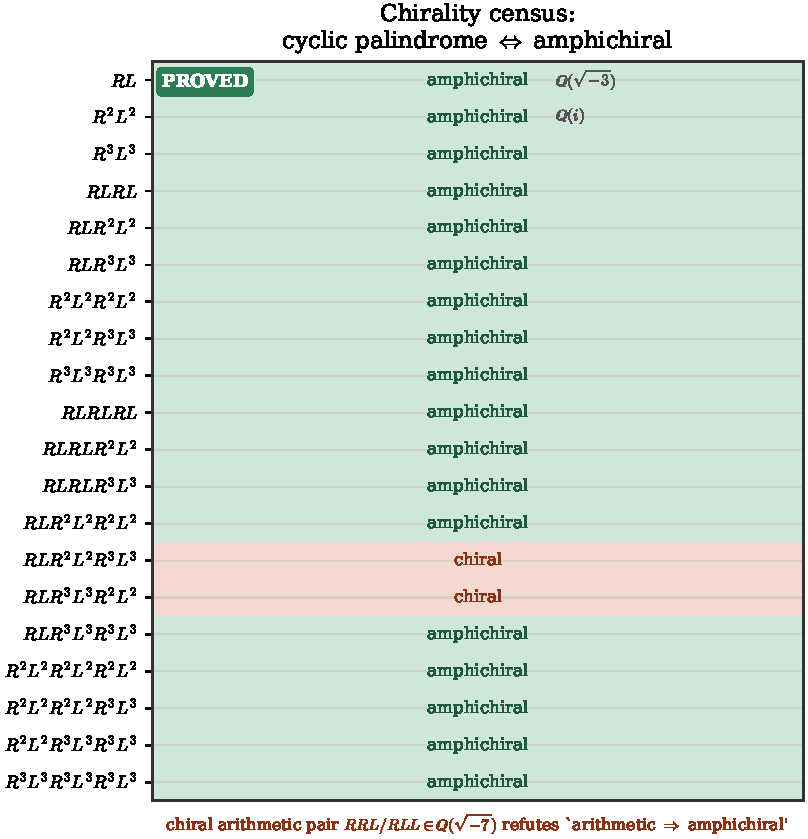
\includegraphics[width=0.56\linewidth]{fig10_chirality_census}
  \caption{The chirality census over metallic-block composites: a sequence is amphichiral
  iff it is a cyclic palindrome. The canonical singles ($RL\in\Q(\sqrt{-3})$,
  $R^2L^2\in\Q(i)$) are self-mirror; the first chiral cases are all-distinct triples.
  \sProved}
  \label{fig:chirality}
\end{figure}

\subsection{The preferred-handedness dichotomy}

Beyond the criterion, the family as a whole cannot prefer a handedness. The mirror of a
metallic composite is another composite of the same pieces, so the family is
\emph{mirror-closed}; chirality, while forced and generic among hyperbolic bundles, is
always either self-mirror (the canonical singles) or mirror-paired (the composites).

\begin{proposition}[\sStruct]\label{prop:dichotomy}
$M_W$ and its mirror $\overline{M_W}$ agree on every orientation-\emph{independent}
invariant. Hence no canonical (orientation-independent) selection principle can prefer a
handedness: a $\kk$-fork is genuine selection, because $\kk$ is orientation-independent,
whereas a chirality-fork is always a convention, because handedness is
orientation-sensitive. The figure-eight is the amphichiral minimum; chirality first
appears strictly above it.
\end{proposition}

\subsection{A refuted shortcut, and what survives}

It is tempting to argue that arithmetic bundles must be amphichiral. This is false. The
chiral mirror pair $RRL/RLL$ --- general $R,L$ words, not metallic-block composites --- is
\emph{fully arithmetic}, with invariant trace field $\Q(\sqrt{-7})$, integral traces, and
a confirming Humbert-volume cross-check. So ``arithmetic $\Rightarrow$ amphichiral'' is
simply wrong; the surviving statement rests on volume-minimality and the dichotomy of
Proposition~\ref{prop:dichotomy}, not on arithmeticity. We record this because it was
found the disciplined way: a numerical result contradicting a cited ``exactly two''
arithmetic chiral count was held until two independent methods agreed and a genuine bug
(reading a leading coefficient at the wrong degree) was fixed. The reading we license is
narrow and exact: \emph{chirality is contingent relative to the metallic minimality
criteria, and no canonical principle prefers a handedness.}

\section{The bridge, and the wall}
\label{sec:bridge}

This is the one section that addresses the motivating question of
Section~\ref{sec:intro}. We hold to the firewall: the mathematics below stands on its own;
the physical reading is labelled and cites the mathematics one way. The result is a pair
--- a forced symmetry bridge and a confirmed dimensional wall --- and we tag each
component as \sForced\ (a mathematical identity), \emph{permitted} (consistent but not
forced), or \emph{rhyme} (a suggestive homonym that is \emph{not} the bridge).

\subsection{The bridge is real}

The once-punctured-torus theory in the class-$S$ construction is the
$\mathcal{N}=2^\ast$ theory (maximally supersymmetric Yang--Mills deformed by an adjoint
mass). Its Coulomb-branch geometry is governed by the \emph{same} Fricke cubic
\eqref{eq:fricke}: the character variety of the once-punctured torus, with the very trace
coordinates of Section~\ref{sec:invariant}. Crucially, the $S$-duality group acts on that
character variety \emph{through the mapping class group}, not merely on the ultraviolet
gauge coupling $\tau$ \cite{allegrettishan2024}.

\begin{theorem}[\sForced, literature-confirmed]\label{thm:bridge}
The $\SL(2,\Z)$ trace-map action of the metallic monodromies on the Fricke character
variety (Proposition~\ref{prop:invariant}) coincides with the $S$-duality /
mapping-class action of the $\mathcal{N}=2^\ast$ class-$S$ theory on its Coulomb branch.
The metallic conjugacy classes, the dilatation eigenvalue $\lambda_m^2$ (the Cantat--Loray
dynamical degree \cite{cantatloray2009}), the fixed slopes, and the Markov fibre are all
reproduced, because it is the same group acting the same way on the same variety
\cite{allegrettishan2024,gmn2013}.
\end{theorem}

This is the widest reach the one-object picture achieves, and it is \sForced, not a
rhyme. The honest caveats are equally precise, and we name them in the same vocabulary:
\begin{itemize}[leftmargin=1.4em]
\item \emph{Forced:} the action on the \emph{character variety} reproduces the anchors of
  Section~\ref{sec:invariant}. This is the bridge.
\item \emph{Rhyme:} ``$\SL(2,\Z)$ acts modularly on the gauge coupling $\tau$'' is the
  well-known $S$-duality \emph{homonym}; it acts on a different space and is \emph{not}
  the trace-map dynamics. We flag it as rhyme precisely so it is not mistaken for the
  bridge.
\item \emph{Rhyme / permitted:} the gauge group is free input and $\mathcal{N}=2^\ast$ is
  non-chiral, so at the level of physical gauge content there is no forced identification.
\end{itemize}
Even the forced bridge is mathematics: it is a symmetry identity, not a crossing to
physics.

\subsection{The wall is confirmed}

That the bridge is real is exactly why the firewall had to be tested hardest: a genuine
symmetry bridge makes a scale-crossing \emph{feel} plausible. So we asked the decisive
question. In the 3d--3d correspondence applied to the figure-eight, does any quantity
carry a \emph{scale} across --- does the complex volume / Chern--Simons invariant enter
the partition function as anything other than a dimensionless exponent?

\begin{theorem}[\sKnown, literature reading]\label{thm:wall}
The complex volume $\widehat c(\rho)=i(\Vol+i\,\CS)$ of an $\SL(n,\C)$ representation is a
dimensionless element of $\C/4\pi^2\Z$ \cite{gtz2015}; in the 3d--3d state integral it
enters only as the exponent saddle, with all dimensionful content carried by the level
$\hbar\leftrightarrow k$ and the squashing radius \cite{dimofte2014,cordovajafferis2013}.
For the figure-eight, $\Vol=2.029883\ldots$ and $\CS=0$: the candidate scale-carrier
vanishes identically. No $\kk$-type or volume-type invariant of the object can source a
physical scale (\fig{fig:bridge}).
\end{theorem}

\begin{figure}[t]
  \centering
  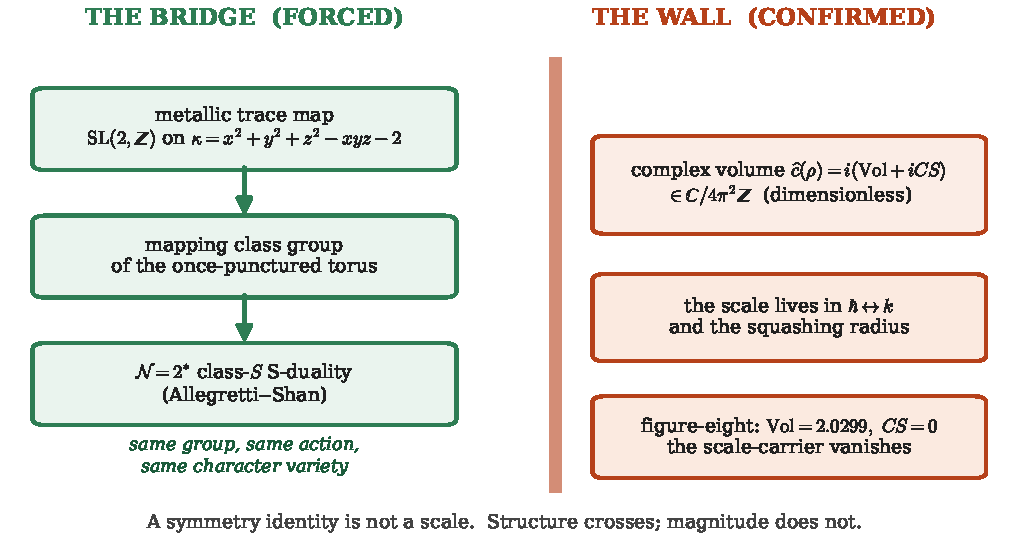
\includegraphics[width=\linewidth]{fig12_bridge_and_wall}
  \caption{The bridge and the wall. \emph{Left (forced):} the metallic $\SL(2,\Z)$
  trace-map symmetry \emph{is} the $\mathcal{N}=2^\ast$ class-$S$ $S$-duality /
  mapping-class action on the Fricke character variety. \emph{Right (confirmed):} the
  complex volume is dimensionless ($\C/4\pi^2\Z$); the scale lives in $\hbar/k$ and the
  squashing radius, and for the figure-eight the scale-carrier $\CS$ vanishes. A symmetry
  identity is not a scale. \sForced\,/\,\sKnown}
  \label{fig:bridge}
\end{figure}

The blade, held to the end: a \emph{symmetry} identification is not a \emph{scale}. ``The
partition function has units'' is not a crossing --- the units are in $\hbar/k$ and the
radius. A crossing would require a dimensionful quantity to attach to the \emph{invariant
itself}, and the literature exhibits the opposite.

\begin{remark}[\sPost]\label{rem:postulated}
There is a sharper, \emph{structural} reason one might give for the wall: a conserved /
topological invariant cannot run, and running is what manufactures a scale; so an object
whose content is a topological invariant cannot, in principle, source one. This is
compelling and was proposed in review, but it has not been put through the project's
verification gate, and so we record it as \sPost\ --- not as the banked result. The banked
wall is the literature reading of Theorem~\ref{thm:wall}.
\end{remark}

\subsection{The seam: the object is open, and closing it is where structure actualizes}

The wall above is about \emph{scale}. A second reading sharpens \emph{where the object's
symmetries break} --- and it turns on a fact we had under-used: the figure-eight is an
\emph{open} object. It is a complement $S^3\setminus K$, defined by what is removed, with a
cusp (boundary torus) as its interface with the exterior. Its amphichirality and
CP-symmetry are \emph{open}-object symmetries; \emph{closing} it --- a Dehn filling --- is
where they break. (Curie's principle, sometimes invoked to argue a symmetric object cannot
self-select an asymmetric outcome, is a \emph{closed}-system statement; it does not bind a
complement, which breaks symmetry through boundary conditions.)

\begin{proposition}[\sKnown\ mathematics, \sForced\ identification]\label{prop:seam}
The figure-eight is the once-punctured-torus bundle with monodromy $A=\big(\begin{smallmatrix}2&1\\1&1\end{smallmatrix}\big)$.
Among its ten exceptional Dehn fillings, the fiber ($0$-slope) filling is the \emph{unique}
$\mathrm{Sol}$ torus bundle, with monodromy exactly $A$ --- the trace-map matrix $A=LR$ of
\S\ref{sec:object} and its torsion ladder $\lvert\det(A^n-I)\rvert$. Every generic filling
is chiral ($\CS\notin\{0,\tfrac12\}$), with the sign law $\CS(p,-q)=-\CS(p,q)$; the
geometric handedness realises complex conjugation of the $\Q(\sqrt{-3})$ trace field --- the
same Galois involution that flips the commutator phase $\kappa=u^2+2=\sqrt3\,e^{\mp i\pi/6}$
between $\pm\pi/6$. The core geodesic of the $(1,n)$ filling has length $\sim 2\pi/n$ (a
Neumann--Zagier ladder); the peripheral $(\mu,\lambda)$ pairing is the Goldman/NZ symplectic
form, a filling a choice of polarization.
\end{proposition}

The mathematics here is classical (Thurston's exceptional surgeries; Garoufalidis--Jeon on
trace-field growth; Goldman and Neumann--Zagier on the symplectic structure); the new part
is the \emph{reading}, and it cuts in a definite direction. Tested across the fillings, the
seam is \emph{selective for the object's own structure} --- the canonical closing re-sees
$A=LR$ --- but a \emph{catalogue for Standard-Model values}: the $E_6$/$\Q(\sqrt{-3})$
arithmetic is \emph{lost} on closing (no filling re-instantiates it, sharpening the
input-$E_6=$output-$E_6$ question toward ``catalogue''), the CP \emph{sign} stays external
(the object is CP-symmetric: it delivers $\pm\pi/6$ symmetrically), the scale \emph{value}
is gapped, and the chiral and dynamical data are not supplied.

\begin{remark}[\sPost]\label{rem:structural-theorem}
This relocates the project's structural theorem to the seam: \emph{the object supplies a
canonical closing and all the dimensionless structure --- the dynamics $A=LR$, the CP
magnitude $\pi/6$ with its forced sign law, the scale ladder $2\pi/n$, the
peripheral-symplectic clock --- while the actualization of a specific Standard-Model-valued
world is not forced}. It is the architecture-not-furniture stance made mechanistic at the
boundary, and it \emph{strengthens} the wall rather than crossing it. As a physics reading
it is \sPost; the mathematics it cites is banked and firewalled.
\end{remark}

\subsection{Where it reaches, and where it stops}

The physics arc closes in the strongest honest place available: a real bridge --- the
object's symmetry \emph{is} the duality action of a gauge theory, forced and
literature-confirmed --- and a confirmed wall --- that bridge carries structure, not
scale. The cosmological-constant question lies on the far side of a wall this structure
does not cross. That pairing is not a failure; it is a result. The work reached across the
widest gap it could, mapped exactly where it arrives and where it stops, and exhibited the
reasons rather than asserting them. What remains after this is mathematics, not physics ---
the subject of the next section.

\section{Discussion: the object's proper name}
\label{sec:discussion}

Stepping back, the four registers of the paper describe one thing, and that thing has a
proper name in mathematics. It is a \emph{metallic-mean Schr\"odinger cocycle} over the
substitution subshift generated by $R^mL^m$, analysed by the Kohmoto--Kadanoff--Tang
trace map, with $\kk$ its Fricke--Vogt invariant \cite{kkt1983,suto1987,baakegrimm2013}.

\subsection{Non-cancellation as positivity}

The founding intuition --- that ``not-nothing'' should be a residue that cannot cancel to
zero --- has an exact translation in this language. Non-cancellation is Fricke--Vogt
positivity $\kk>2$; this is precisely the hyperbolicity condition of the trace map; and
that hyperbolicity is exactly the condition for the associated one-dimensional aperiodic
Schr\"odinger operator to have purely singular-continuous spectrum supported on a Cantor
set \cite{suto1987}. Figure~\ref{fig:cantor} shows that spectrum for the golden case: as
the coupling grows, gaps open on every scale and the spectrum becomes a Cantor set --- the
operator-theoretic shadow of the metallic dynamics. This is genuine, observed physics ---
aperiodic order, the spectral theory of quasicrystals --- and it is emphatically
\emph{not} fundamental physics: there is no gauge theory here, no constant of nature, no
spacetime. It is the honest physical home of the object, and it sits comfortably on the
mathematics side of the firewall.

\begin{figure}[t]
  \centering
  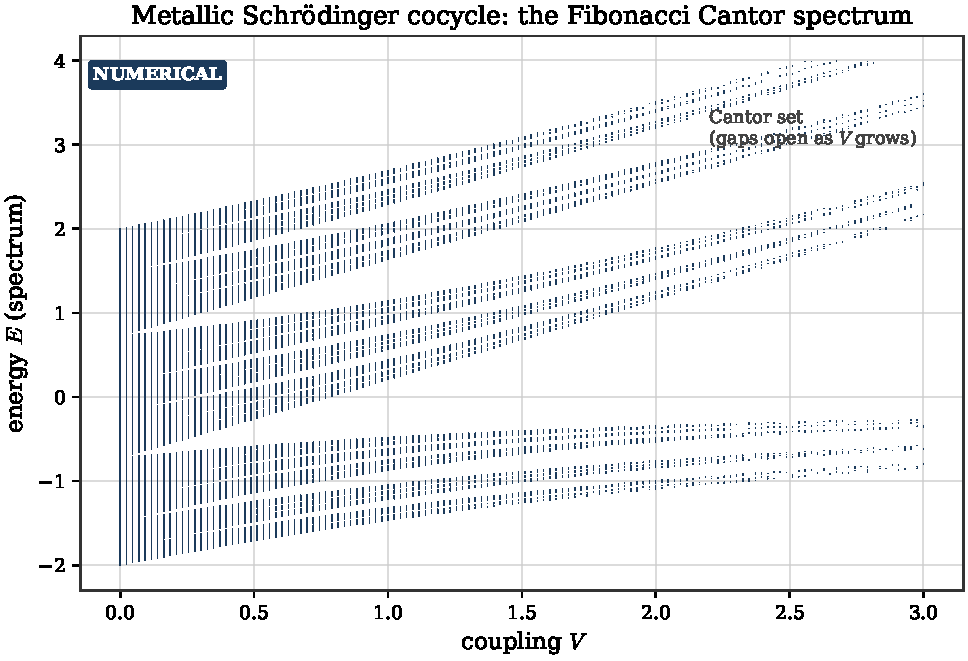
\includegraphics[width=0.86\linewidth]{fig11_cantor_spectrum}
  \caption{The object's proper name. The spectrum of the Fibonacci (golden-mean)
  Schr\"odinger operator as a function of the coupling $V$: a Cantor set whose gaps are
  organised by the trace-map dynamics. Non-cancellation $\kk>2$ is exactly the
  hyperbolicity that produces it. \sNum}
  \label{fig:cantor}
\end{figure}

\subsection{The obstruction map}

Reading the paper as a whole, the object is bounded by a small number of clearly located
walls, and naming them is as much a result as the bridges. The motivating ambition met
obstructions at six recurring places: a \emph{source} (what generates the family is a
chosen minimality, not a derived necessity); a \emph{selector} (no principle forces the
golden seed over the others); a \emph{measure} (the character variety parametrises
possibilities, it does not weight them); a \emph{unit} (the invariants are dimensionless,
Section~\ref{sec:bridge}); a \emph{dictionary} (the class-$S$ bridge is a symmetry
identity, not a field-content map); and an \emph{observable} (nothing in the construction
inserts a measurement). The firewall is the discipline of mapping these walls honestly,
and the bridge/wall pairing of Section~\ref{sec:bridge} is the sharpest instance: the
object reaches as far as a symmetry and stops exactly at a scale.

\subsection{What the object is, and is not}

It is a small, self-generating mathematical object that turned out to know about knots
(the figure-eight $A$-polynomial), Lie theory (the Dickson tower and the opposition
involution), aperiodic order (the Cantor spectrum), and a gauge theory's duality (the
class-$S$ bridge). It is not a theory of physical values; the firewall holds, and we have
exhibited why. The most honest summary is that the object knows, precisely, where its own
reach ends --- and that this boundary, mapped exactly, is the paper's real subject.

\section{Open problems and method}
\label{sec:open}

\subsection{Open problems}

\begin{enumerate}[leftmargin=1.6em]
\item \textbf{The general-$n$ tower from first principles.} Prove the Dickson
  factorisation (Theorem~\ref{thm:tower}) for all $n$ by exhibiting the functorial
  $\Sym(W)$ construction of \eqref{eq:symw} --- equivalently, assemble the bounded
  rank-one $e_2/\Lambda^2$ closure into the exact trace map as a natural transformation.
  This is the paper's principal open theorem; the obstruction is the doubly-degenerate
  $\chi(M^2)^2$ sector that first appears at $n=5$.
\item \textbf{The novelty gate on $L=-M^4$.} Settle whether the $\SL(4)$ relation
  (Theorem~\ref{thm:m4l}) and the family $L=(-1)^{n-1}M^n$ are new within the
  Bergeron--Falbel--Guilloux / Garoufalidis--Thurston--Zickert frameworks
  \cite{bfg2014,gtz2015}, by a specialist read. Until then the result stays \sGated.
\item \textbf{The principal $\SL(5)$ representation.} Either locate it (against the forced
  degeneracy of Section~\ref{sec:knot}) or prove it cannot exist as an irreducible bundle
  representation --- which would confirm that ``exponent $=$ rank'' is exactly an
  $n\in\{3,4\}$ phenomenon.
\end{enumerate}

\subsection{Method and reproducibility}

The results above were produced under a fixed verification discipline, which we describe
because it is part of what makes a wide-ranging exploration trustworthy. Every figure in
this paper is regenerated by a single deterministic script
(\texttt{figures/gen\_figures.py}); the symbolic and finite-field computations behind
Theorems~\ref{thm:tower}, \ref{thm:m4l} and \ref{thm:complete} are reproducible from the
project's probe code and its committed data artifacts. Five guard-rails, applied
throughout, are worth naming:
\begin{itemize}[leftmargin=1.4em]
\item \emph{Run the control.} A number that reproduces exactly may still be
  interpretively false; vary the causal variable and confirm the effect tracks it.
\item \emph{Filter the reducible locus} before counting character-variety points, and
  test irreducibility with a criterion valid for non-semisimple representations (Burnside,
  not the Schur commutant --- see Section~\ref{sec:knot}).
\item \emph{Generic $\ne$ discriminating.} Check the null case; a feature present
  everywhere distinguishes nothing.
\item \emph{State results twice:} the bare mathematical statement, and --- separately
  tagged, never contaminating the first --- any physical reading
  (Remark~\ref{rem:postulated}).
\item \emph{Check for vacuity.} Before using a target, exhibit a case in which it could
  fail; a property that cannot fail is not a property.
\end{itemize}
These are not stylistic preferences. Each caught a concrete error in the work reported
here: a leading-coefficient bug in the chirality count (Section~\ref{sec:chirality}), a
false irreducibility verdict from the Schur commutant (Section~\ref{sec:knot}), and the
over-statement of a conversational sharpening, demoted to \sPost\
(Remark~\ref{rem:postulated}). The discipline, more than any single theorem, is what we
would ask a reader to trust.

\subsection*{Acknowledgements}
This work was carried out with AI-assisted computation and exposition under the
verification discipline described above; all results are reproducible from the cited code
and data.

\appendix

\section{Proof sketches}
\label{app:proofs}

We collect the load-bearing computations in outline; full symbolic scripts and
finite-field certificates are in the project's probe code.

\subsection{The Fricke identity \texorpdfstring{$\kk=4I_{\mathrm{FV}}+2$}{kappa = 4 I + 2}}
\label{app:kappa}

With $A,B\in\SL(2,\C)$ and $x=\tr A,\ y=\tr B,\ z=\tr AB$, the Cayley--Hamilton relation
$A^2=(\tr A)A-I$ and the trace identity $\tr(AB)+\tr(AB^{-1})=\tr A\,\tr B$ give, after a
direct expansion, $\tr[A,B]=\tr(ABA^{-1}B^{-1})=x^2+y^2+z^2-xyz-2$, which is
\eqref{eq:fricke}. Substituting the half-trace normalisation $x=2X,\,y=2Y,\,z=2Z$ yields
$\kk=4(X^2+Y^2+Z^2-2XYZ-1)+2=4I_{\mathrm{FV}}+2$, which is \eqref{eq:kfv}. That the two
Dehn-twist automorphisms preserve $\kk$ is checked by composing the explicit substitutions
$(x,y,z)\mapsto(x,\,z,\,xz-y)$ and its partner and confirming $\kk$ is fixed; the
verification is a finite symbolic identity.

\subsection{The $\SL(4)$ Dickson factorisation by CRT/$\Fp$}
\label{app:crt}

Direct symbolic computation of the $15\times15$ Jacobian $J(m)$ over $\Z[m]$ is feasible
but heavy; we instead reconstruct it by interpolation. For each prime $p$ in a fixed set
and each integer $m_0$ in a range exceeding the total degree, the numeric Jacobian
$J(m_0)\bmod p$ is assembled and its characteristic polynomial computed. Lagrange
interpolation in $m_0$ recovers the coefficients mod $p$; the Chinese Remainder Theorem
and rational reconstruction across the primes recover them over $\Q$. The resulting
characteristic polynomial factors exactly as in Theorem~\ref{thm:tower}; the factorisation
$(t-1)^2(t+1)\prod\chi(\pm M^k)$ is then confirmed against the Dickson catalogue
symbolically. The technique (modular interpolation $+$ CRT $+$ rational reconstruction) is
standard computational algebra; only its application here is the project's.

\subsection{$L=-M^4$ by ideal elimination}
\label{app:m4l}

On the principal $A$-spectrum $\{1,1,\omega,\omega^2\}$ one writes the bundle relation
$B\,\rho(\varphi)\,B^{-1}=\rho(\varphi)^{\text{conj}}$ and eliminates $B$, collapsing the
defining equations to an ideal in the entries of the coupling block $t$. On the
rank-two stratum $t_{11}=\omega\,t_{22}$ the solution set is a four-parameter family, and
on it the commutator longitude satisfies the polynomial identity
$[A,B]\cdot\det(t)^2=-\det(t)\cdot\mu^4$ with $\mu=A^{-1}t$ the meridian; clearing the
common factor $\det(t)\ne0$ on the irreducible stratum gives $L=-M^4$ at the level of
eigenvalues. No division is performed before the non-vanishing of $\det(t)$ is established,
and no numerics enter. Completeness (Theorem~\ref{thm:complete}) is the separate
finite-field Burnside classification described in Section~\ref{sec:knot}.

\subsection{Figure reproduction}
\label{app:figs}

All figures are produced by \texttt{figures/gen\_figures.py} under the canonical Python
environment. Figures~\ref{fig:tower} and \ref{fig:strat} read committed data artifacts
(the symbolic $\SL(4)$ Jacobian and the finite-field stratification certificate);
Figures~\ref{fig:metallic}, \ref{fig:fricke}, \ref{fig:dynamics}, \ref{fig:opp},
\ref{fig:apoly}, \ref{fig:slope}, \ref{fig:chirality}, \ref{fig:cantor} and
\ref{fig:bridge} are recomputed in-script and are deterministic. Each figure carries the
proof-status badge of the result it depicts, mirroring the badges in the text.


\bibliographystyle{plain}
\bibliography{refs}

\end{document}
